\section{Background}


\begin{figure}
\centering
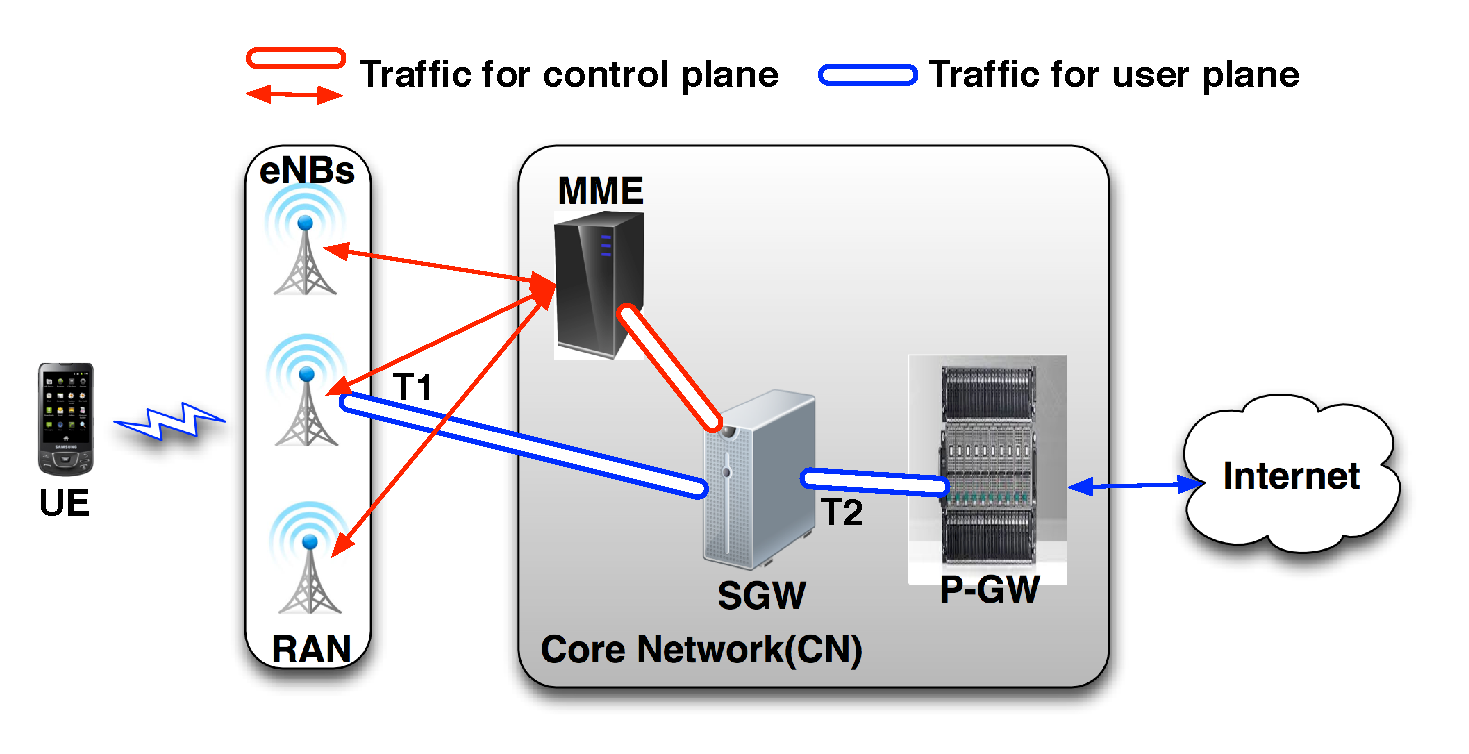
\epsfig{file=./figure/mobi_basic, height=3.5cm , width=8cm}
\caption{LTE/EPC Architecture}
\label{fig:mobi_basic}
\end{figure}

In this section, we briefly introduce the cellular network infrastructure, especially LTE and EPC architecture and protocol. 
Figure 1 shows LTE and EPC architecture which is made up of two components: Radio Access Network(RAN) and the Core Network(CN). 

 The RAN consists of eNodeBs ( enhanced NodeBs ) which are connected to User Equipment (UE) like cellphone  through radio link and sends the packet to Serving Gateway(SGW).  In addition, it manages radio resource and supports the intra-LTE mobility. The EPC is a framework which consists of Mobility Management Entity(MME), Serving Gateway(SGW), and Packek Data Network Gateway(PGW). The MME is a key component for performing UE registration, authentication, and mobility management. Also, it is responsible for the tracking and the paging of UE in idle-mode. It does not participate in packet forwarding. The SGW and the PGW are mainly responsible for routing/forwarding the data packets from all UE to the external network and vice versa. Besides packet forwarding, the SGW works as an anchor point in case of handover between eNodeBs and reserves buffers for paging functionality. The PGW performs the most functions among components in EPC such as IP address allocation to UE, charging, packet filtering, and supporting Quality of Service(QoS) according to the users’ data plan.

When the user attaches the cellular network, the components exchange many control messages, which are shown as red line in Figure~\ref{fig:mobi_basic} and called control plane.
After finishing exchanging control message, the connection between UE and cellular network is established with two separate tunnels.
After establishing the connection, the UE can send and receive the packet via tunnels which called user plane and shown as blue lines in Figure~\ref{fig:mobi_basic}. 

\begin{figure}
\centering
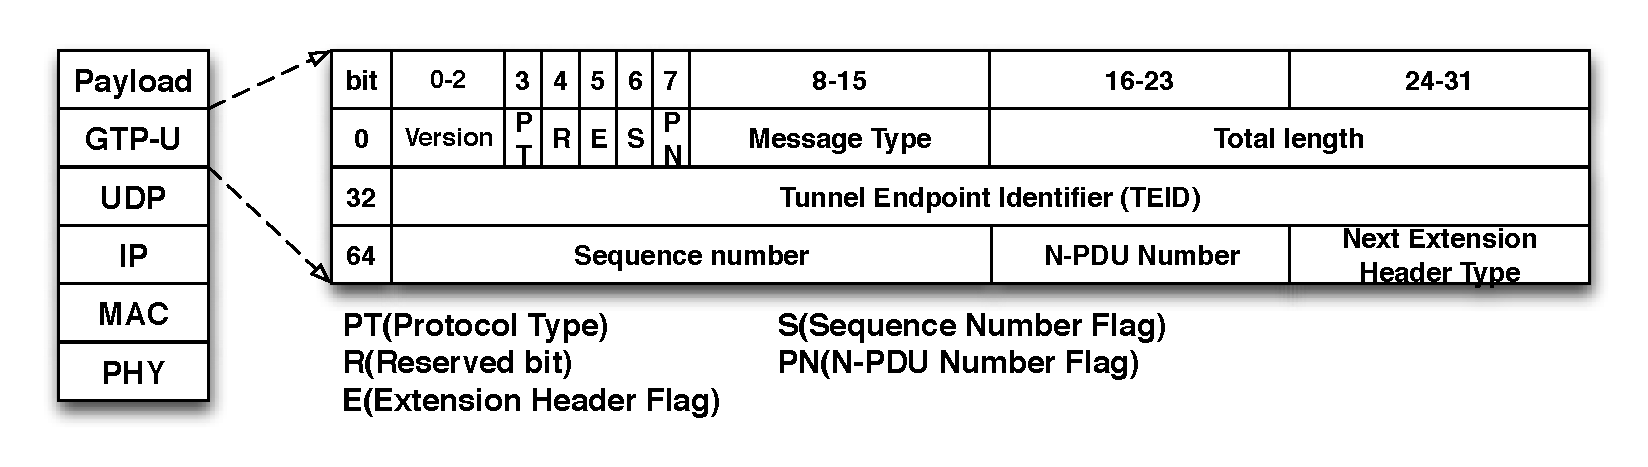
\epsfig{file=./figure/Protocol_Stack , height=3.5cm , width=8cm}
\caption{Protocol stack and GTP-U packet}
\label{fig:gtp-u}
\end{figure}

The tunnel between two componets is represented by GPRS Tunneling Protocol(GTP). The cellular network uses GTP for data transfer as well as for supporting mobility, quality of service per user. The Figure~\ref{fig:gtp-u} shows the protocol stack and GTP-U packet header. Each component in LTE and EPC architecture communicates with each other by using this protocol stack. For example, the enodeb encapsulates the packet received by UE before sending the packet to SGW and forwards encapsulated packet to SGW.  After SGW receives the encapsulated packet from enodeb, it decapsulates, re-encapsulates and sends it to PGW. The encapsulation and decapsulation process is to replace the protocol layers depicted by gray boxes in Figure ~\ref{fig:gtp-u}. However, the IP and payload layer above GTP-U layer does not change in cellular network and PGW finally decapsulates the packet and forwards it to external network. The packet from external network also work same way. Each tunnel can be distinguished by the unique Tunnel EndPoint Identifier(TEID) and when each component encapsulates the packet, TEID field is set by the destination TEID in GTP-U packet header shown in Figure~\ref{fig:gtp-u}.
